%!TEX ROOT = thesis.tex
\chapter{METHODOLOGY}

The implementation of this project is split into five different steps namely Data Collection, Data Preprocessing, Model Design and Implementation, Model Evaluation and Model Refinement. The general flow of the research methodology can be seen in figure \ref{fig:flowchart1}.

\FloatBarrier
\begin{figure}[!h]
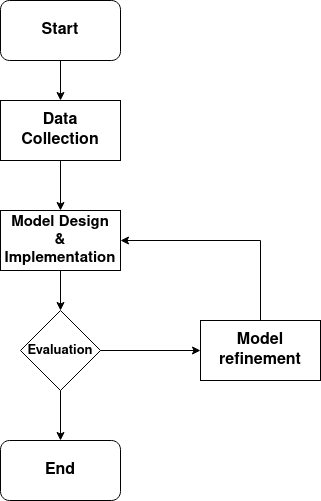
\includegraphics[width=7.5cm, height=8.5cm]{images/flowchart1.png}
\centering
\caption{Flowchart of Proposed Research Methodology}
\label{fig:flowchart1}
\end{figure}


\section{Data Collection}

There were 12 different datasets considered at the beginning of this project and their details can be found in Chapter 2. In the end, we decided to choose LoveDA dataset \cite{loveda} because of several reasons. The first reason is it has one of the lowest spatial resolution with 0.3m. The second reason is it has a total of 5,987 samples which we considered as a good number of samples. Te third reason is the images in LoveDA dataset is actually collected satellites unlike severeal other dataset that is a mixed of images collected through satellites and drones. The final reason is the images on LoveDA comes in PNG format which is much easier to work with compared to some other dataset that comes in GeoTIFF format. Although GeoTIFF carry more information, we concluded that the time and effort required to process and train models using GeoTIFF format is too much.

LoveDA dataset was introduced in Chapter 2 but here we are going to give a more detailed statistical analysis on the dataset. Table \ref{tab:class-loveda} explains the description of the classes in the dataset.

\begin{table}[!h]
\begin{tabular}{|l|l|}
\hline
\multicolumn{1}{|c|}{\textbf{Classes}} & \multicolumn{1}{c|}{\textit{\textbf{Description}}}                                                                                \\ \hline
\textit{\textbf{Background}}           & Any objects that don't really belong in the rest of the class.                                                                    \\ \hline
\textit{\textbf{Building}}             & Include objects such as houses, schools, farmhouses                                                                               \\ \hline
\textit{\textbf{Road}}                 & Include tar roads and dirt roads.                                                                                                 \\ \hline
\textit{\textbf{Water}}                & Include rivers, lakes, sea, pools and drains.                                                                                     \\ \hline
\textit{\textbf{Barren}}               & \begin{tabular}[c]{@{}l@{}}Unused land that is not used for any residential,\\ commercial or agriculture activities.\end{tabular} \\ \hline
\textit{\textbf{Forest}}               & Forest.                                                                                                                           \\ \hline
\textit{\textbf{Agriculture}}          & Farms.                                                                                                                            \\ \hline
\end{tabular}
\caption{Classes Description for LoveDA Dataset.}
\label{tab:class-loveda}
\end{table}

Each pixel in the dataset is labelled as it is made specifically for sematic segmentation task. The images in LoveDA dataset are separated into two groups; the rural images and the urban images. Each of the group is already splitted into a training set, a validation set and a testing set. The structure of the dataset is shown in figure \ref{fig:loveda-structure} .

\FloatBarrier
\begin{figure}[!h]
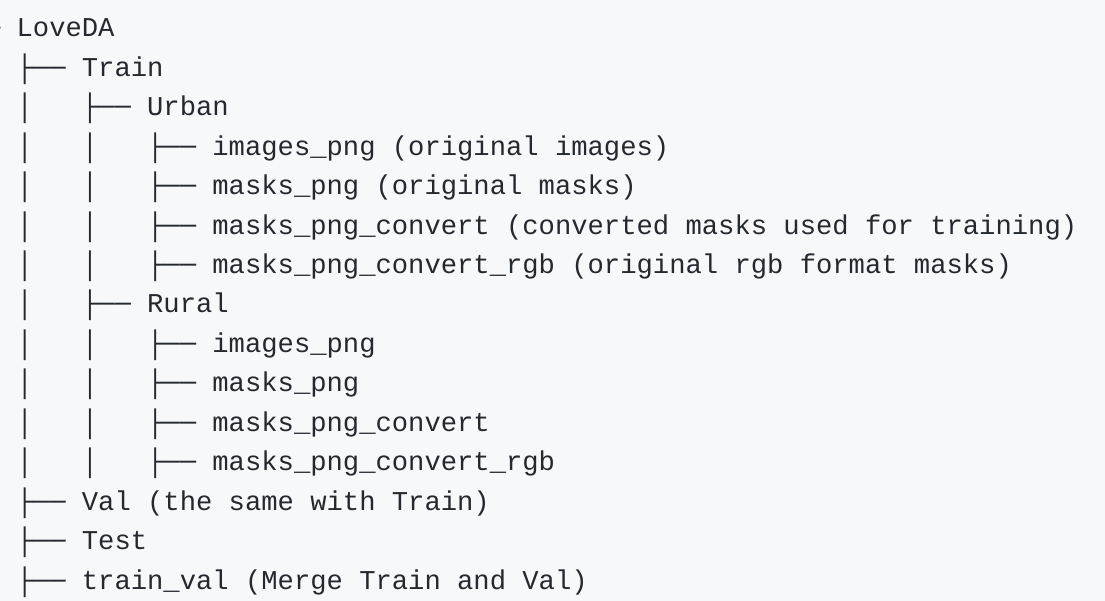
\includegraphics[width=7.5cm, height=4.5cm]{images/loveda-structure.png}
\centering
\caption{The Structure of LoveDA Dataset}
\label{fig:loveda-structure}
\end{figure}

Figure \ref{fig:boxplot-rural-train}, \ref{fig:boxplot-urban-train}, \ref{fig:boxplot-rural-test} and \ref{fig:boxplot-urban-test} show the boxplots of the classes in the training and test set while figure \ref{fig:barplot-rural-train}, \ref{fig:barplot-urban-train}, \ref{fig:barplot-rural-test} and \ref{fig:barplot-urban-test} show the distribution of the same datasets. We observed that there is definitely class imbalanced in all four sets of the data. Rural areas have more agriculture and forest as expected. Urban area have more roads and buildings as the buildings in urban area are bigger and situated closely together while the roads in urban area are generally wider than the ones in rural area. Water are often exist in the form of large-scale rivers, drains or lakes in the urban scenes, while small ponds and ditches are more common in the rural scenes. In urban area, the agricultural part is often found in the gaps between the buildings while the rural area have a more continuous and large agricultural lands.

There are two concerning observations from the graphs. The first one being the amount of agriculture in the urban test dataset is larger than expected. the second concern being both rural and urban areas have a very large amount of background area and the background have very different meaning in these two areas. The background in urban area are usually the sidewalks, parking lots and parks while the background in rural area are usually the unused gaps between agricultural area. 

\FloatBarrier
\begin{figure}[!h]
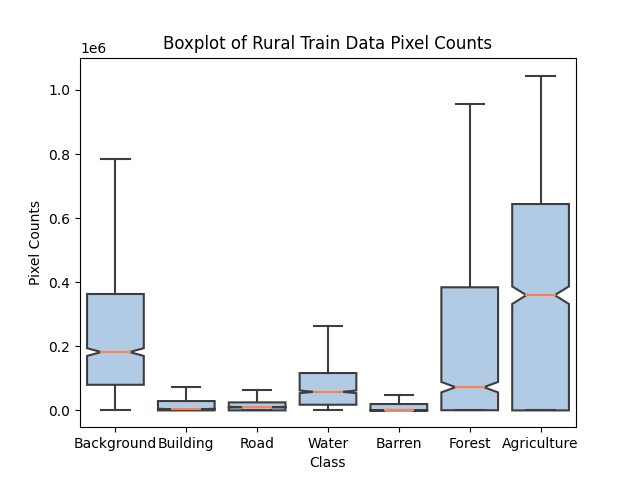
\includegraphics[width=15.0cm, height=8.5cm]{images/rural train boxplot.png}
\centering
\caption{Boxplot of the Pixel Counts of the Rural Train Dataset}
\label{fig:boxplot-rural-train}
\end{figure}

\begin{figure}[!h]
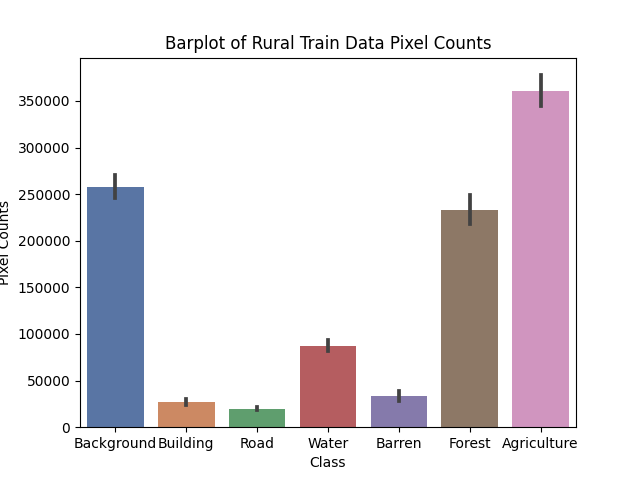
\includegraphics[width=15.0cm, height=8.5cm]{images/rural train barplot.png}
\centering
\caption{Barplot of the Pixel Counts of the Rural Train Dataset}
\label{fig:barplot-rural-train}
\end{figure}

\begin{figure}[!h]
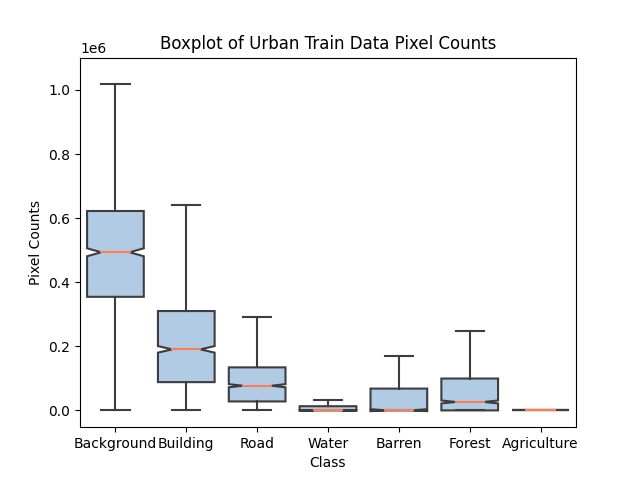
\includegraphics[width=15.0cm, height=8.5cm]{images/urban train boxplot.png}
\centering
\caption{Boxplot of the Pixel Counts of the Urban Train Dataset}
\label{fig:boxplot-urban-train}
\end{figure}

\begin{figure}[!h]
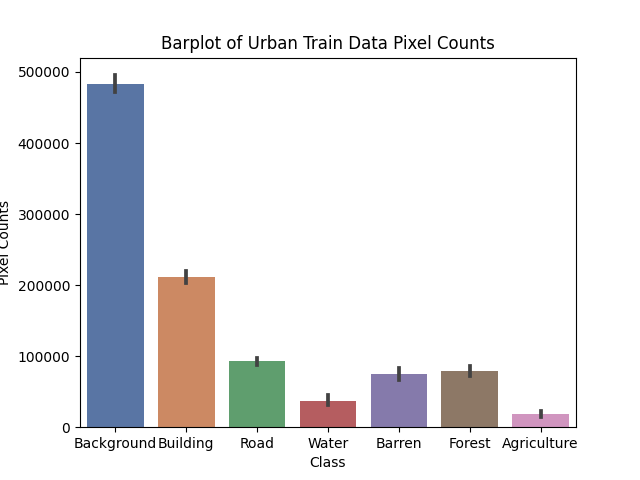
\includegraphics[width=15.0cm, height=8.5cm]{images/urban train barplot.png}
\centering
\caption{Barplot of the Pixel Counts of the Rural Train Dataset}
\label{fig:barplot-urban-train}
\end{figure}


\begin{figure}[!h]
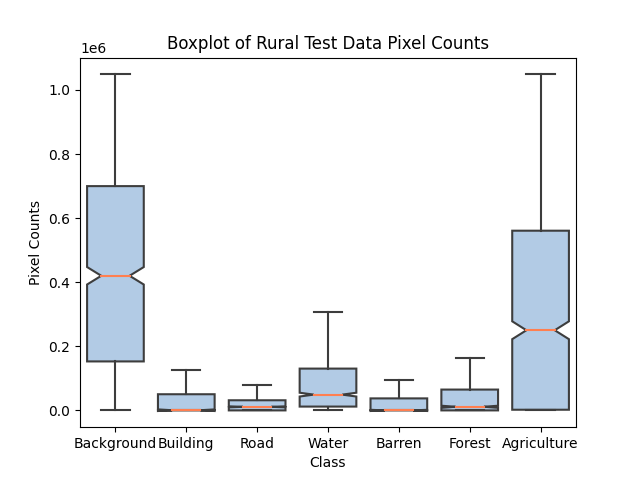
\includegraphics[width=15.0cm, height=8.5cm]{images/rural test boxplot.png}
\centering
\caption{Boxplot of the Pixel Counts of the Rural Test Dataset}
\label{fig:boxplot-rural-test}
\end{figure}

\begin{figure}[!h]
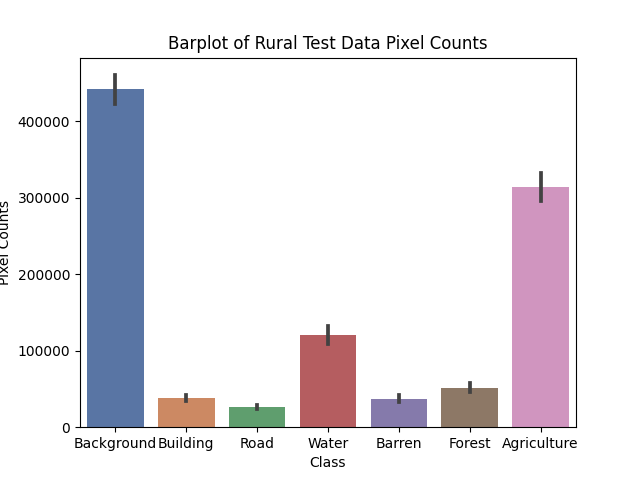
\includegraphics[width=15.0cm, height=8.5cm]{images/rural test barplot.png}
\centering
\caption{Barplot of the Pixel Counts of the Rural Test Dataset}
\label{fig:barplot-rural-test}
\end{figure}


\begin{figure}[!h]
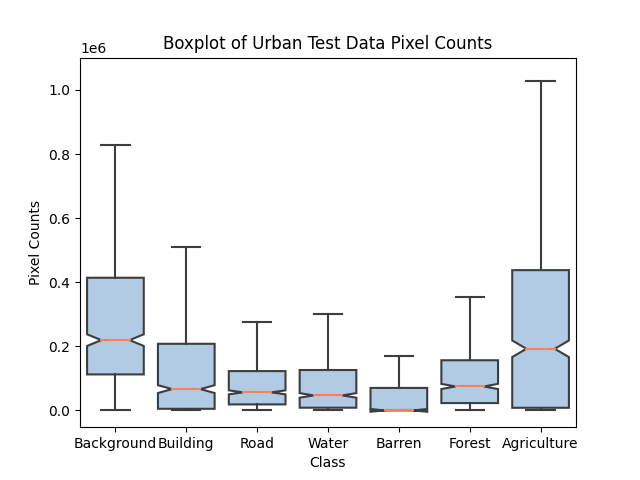
\includegraphics[width=15.0cm, height=8.5cm]{images/urban test boxplot.png}
\centering
\caption{Boxplot of the Pixel Counts of the Urban Test Dataset}
\label{fig:boxplot-urban-test}
\end{figure}

\begin{figure}[!h]
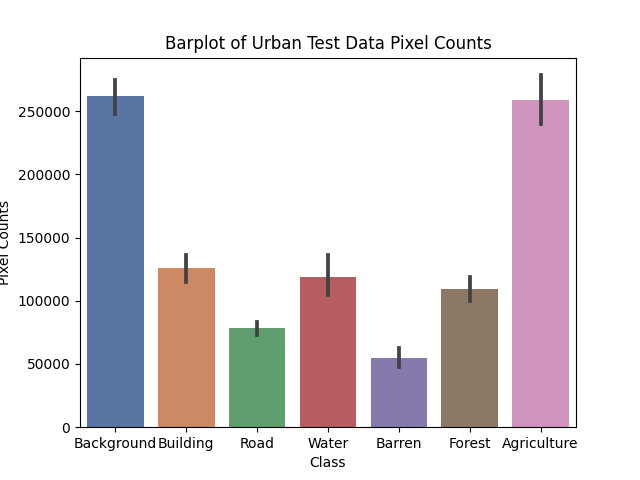
\includegraphics[width=15.0cm, height=8.5cm]{images/urban test barplot.png}
\centering
\caption{Barplot of the Pixel Counts of the Urban Test Dataset}
\label{fig:barplot-urban-test}
\end{figure}

\FloatBarrier


\section{Data Preprocessing}







\section{Model Design and Implementation}

\section{Model Evaluation}

\section{Model Refinement}
